\documentclass[10pt,letterpaper]{book}
\usepackage[utf8]{inputenc}
\usepackage{amsmath}
\usepackage{amsfonts}
\usepackage{amssymb}
\usepackage{graphicx}
\usepackage{epstopdf}
\author{Jason Milldrum, NT7S.} %LaTeX don't like several authors afaik.

\title{Radio Measurements For The Amateur}

\newcommand*{\titleGM}{\begingroup % Create the command for including the title page in the document
\hbox{ % Horizontal box
\hspace*{0.15\textwidth} % Whitespace to the left of the title page
\rule{1pt}{\textheight} % Vertical line
\hspace*{0.05\textwidth} % Whitespace between the vertical line and title page text
\parbox[b]{0.75\textwidth}{ % Paragraph box which restricts text to less than the width of the page

{\noindent\Huge\bfseries Radio Measurements for the Amateur}\vspace{30pt}[2\baselineskip] % Title
{\large \textit{\today}}\vspace{30pt}[4\baselineskip] % Tagline or further description
{\Large \textsc{Jason Milldrum, NT7S}} % Author name
{\Large \textsc{Thomas S. Knutsen, LA3PNA}} % 2. Author name

\vspace{0.6\textheight} % Whitespace between the title block and the publisher
{\noindent Etherkit}\vspace{30pt}[\baselineskip] % Publisher
{\noindent https://github.com/NT7S/RadioMeasurements}\vspace{30pt}[\baselineskip] % Publisher
}}
\endgroup}
\begin{document}
\titleGM % Include title page
\chapter{Introduction}
blah
\chapter{Glossary}
\begin{tabular}{ll}
AF & Audio Frequency \vspace{30pt} 
CW & Continuous Wave, i.e. a single tone \vspace{30pt}
DUT & Device Under Test \vspace{30pt}
RMS & Root-mean-square \vspace{30pt}
\end{tabular} 
\chapter{Test Equipment}
blah
\chapter{Receiver Measurements}
\section{Minimum Discernible Signal (MDS)}
\subsection*{Overview}
The purpose of this test is to measure the lowest-level CW signal which can be detected by a receiver. This is defined as a signal input at the receiver antenna port which produces the same amount of AF power output as the intrinsic background noise of the receiver. In other words, when a signal at the MDS level is applied to the antenna port, a 3 dB increase in output power is measured over the receiver's internal noise level measurement.
\subsection*{Equipment List}
\begin{itemize}
	\item RF Signal Generator
	\item 100 dB Step Attenuator (at least 1 dB steps required)
	\item AC RMS Voltmeter (preferably with dB scale)
	\item AF Monitor Amplifier or 8 $\Omega$ Resistive Load
\end{itemize}
\subsection*{Test Setup}
\begin{figure}
\centering
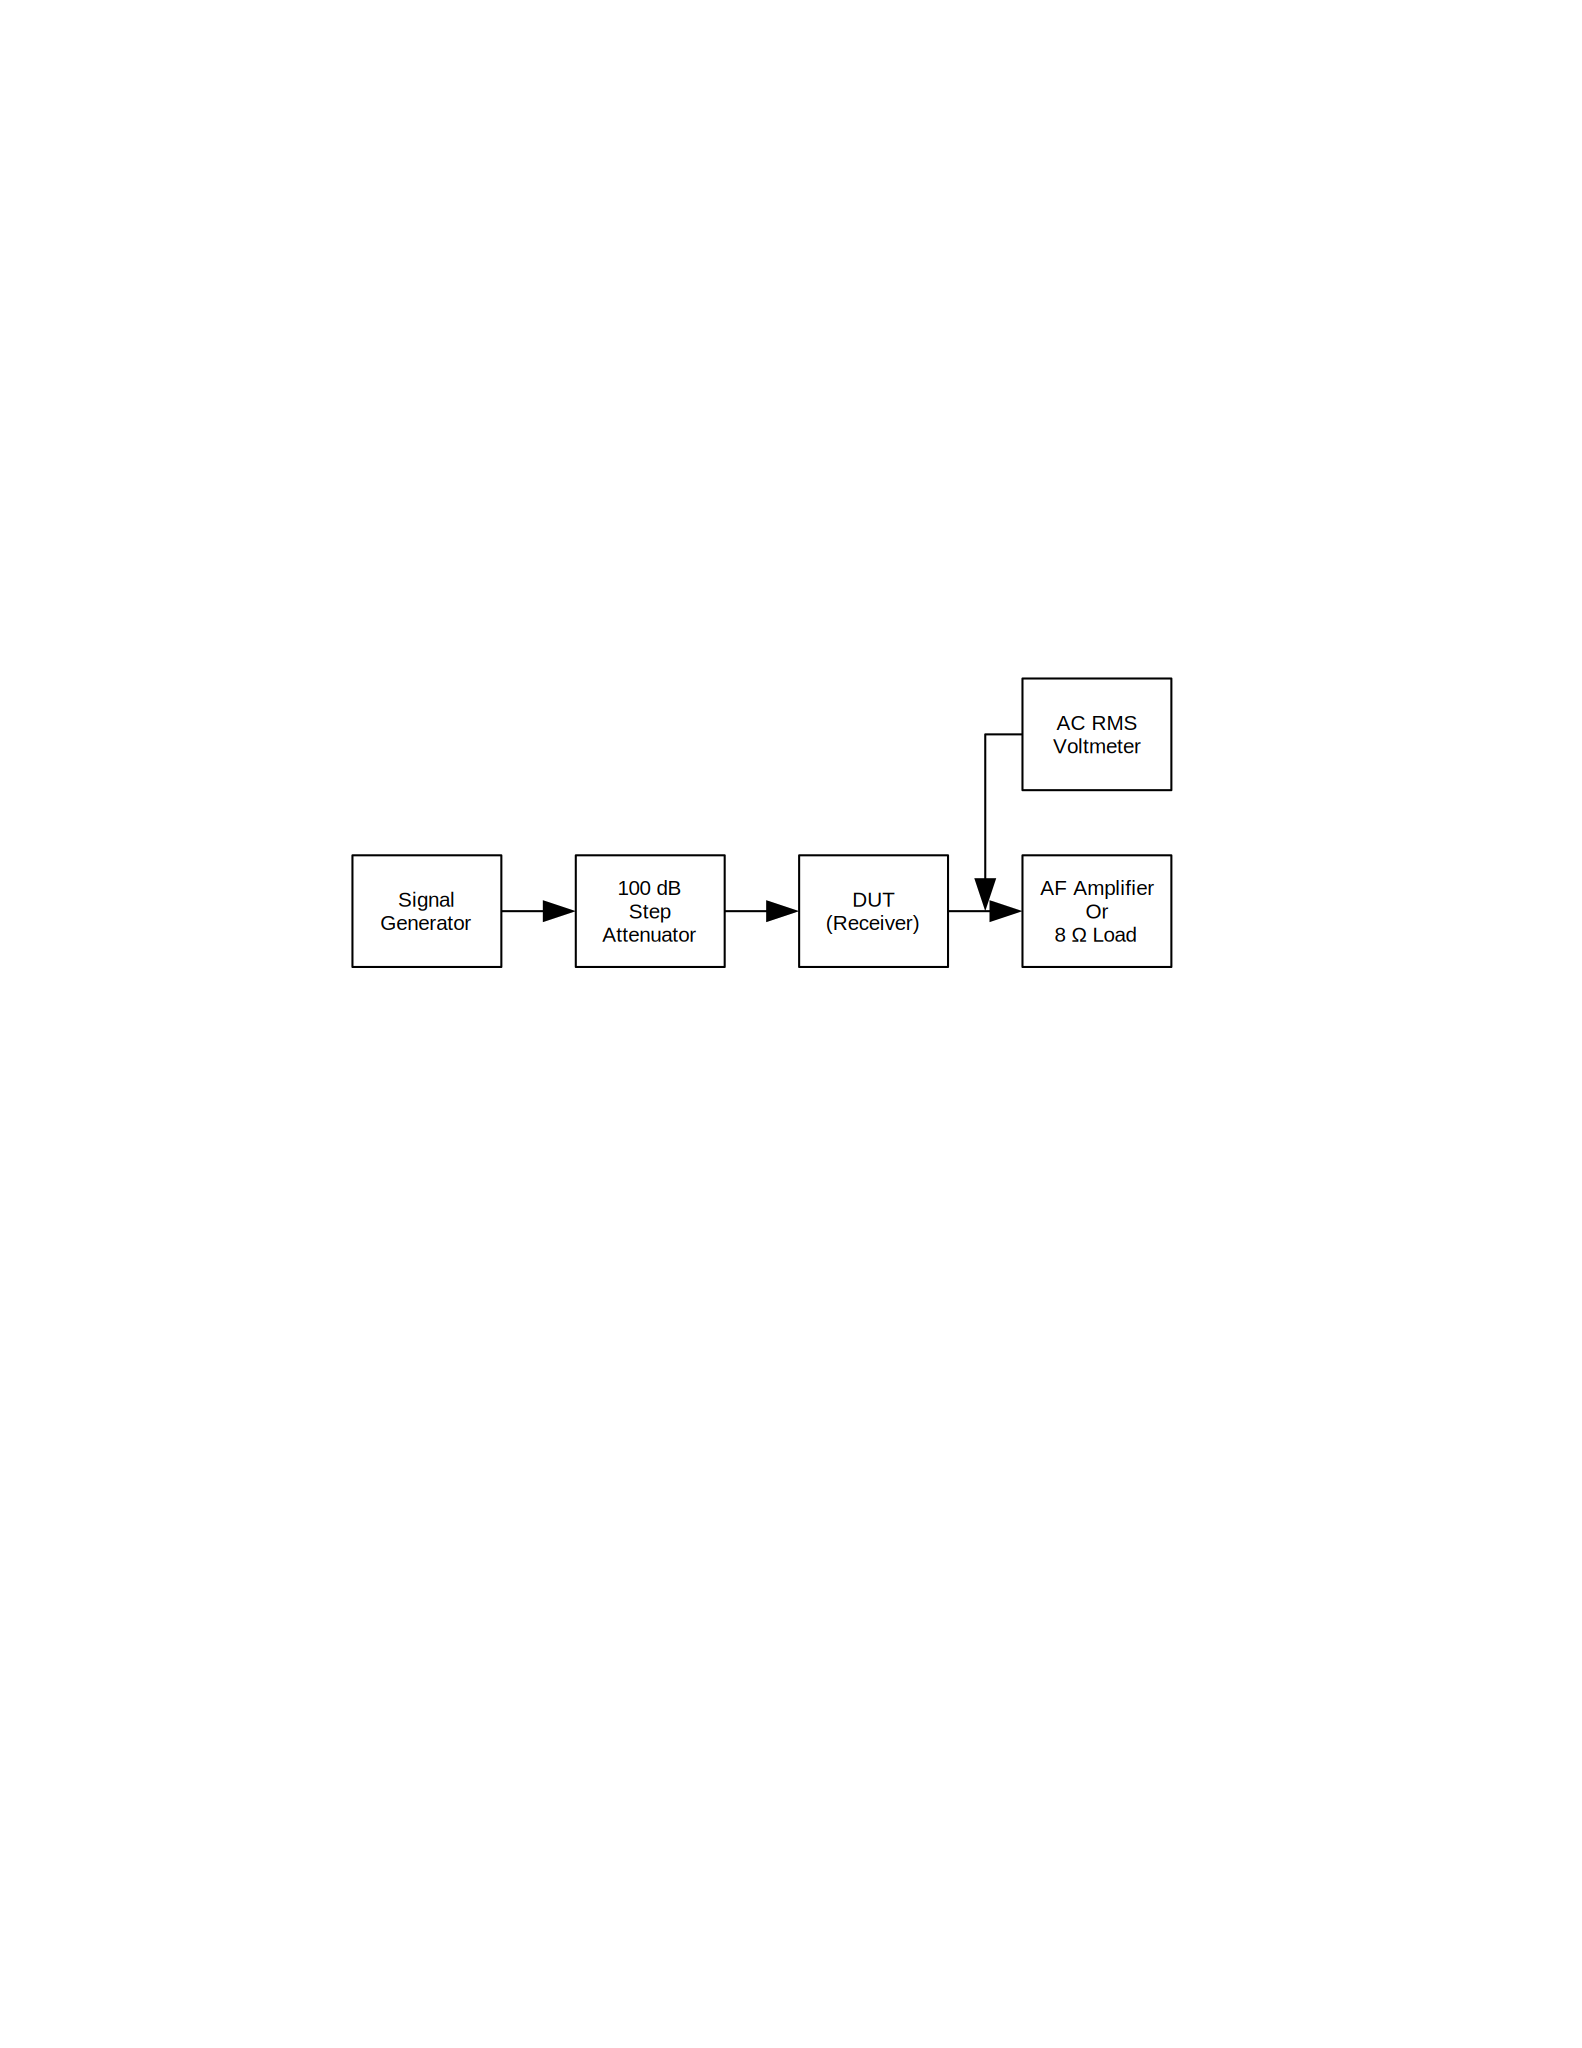
\includegraphics[scale=1]{Illustrations/MDSSetup}
\caption{MDS Measurement Setup}
\end{figure}
\subsubsection*{Required Cabling}
\begin{itemize}
	\item 2 --- 50 $\Omega$ jumper cables \vspace{30pt}
		Usually BNC Male-to-BNC Male
	\item 1 --- audio jumper cable \vspace{30pt}
		Varies depending on the connectors on your receiver and AF amplifier or load
	\item 1 --- set of voltage probe test leads \vspace{30pt}
		Your choice of connector for measuring AC RMS voltage output
\end{itemize}
\subsubsection*{Connections}
\emph{Make sure all equipment is powered off before making any connections.}
\begin{itemize}
	\item Connect the signal generator output to one port of the step attenuator using a 50 $\Omega$ jumper cable.
	\item Connect the other port of the step attenuator to the DUT (receiver) using a 50 $\Omega$ jumper cable.
	\item Connect the audio output of the DUT (receiver) to the AF amplifier or 8 $\Omega$ load using an audio jumper cable.
	\item Connect the AC RMS voltmeter probes to the properly loaded audio output of the DUT (receiver).
\end{itemize}
\subsubsection*{Presets}
\begin{itemize}
	\item Turn ON the signal generator but make sure that the output is OFF. Set the output level to -50 dBm (if you are able to). Set the output frequency to the desired test frequency.
	\item Set the step attenuator for -40 dB. This will give an initial test signal level of -90 dBm. If you are not able to set your signal generator to -50 dBm, set the step attenuator to give you -90 dBm of test signal output.
	\item Turn ON the AF amplifier.
	\item Turn ON the DUT (receiver) and set for the desired measurement band and frequency. Set the AF gain (volume) control fully-counterclockwise (no AF output), then set to an appropriate level for normal listening. If your receiver has AGC, disable it.
	\item Turn ON the AC RMS voltmeter. Set the meter scale as necessary.
\end{itemize}
\subsection*{Test Procedure}
\begin{enumerate}
	\item Turn ON the signal generator output. You should hear a CW tone from the AF amplifier.
	\item Fine-tune the tune control of the DUT (receiver) until the CW tone is centered in the passband and is at maximum level.
	\item Turn OFF the signal generator output.
	\item 4. Note the reading of the AC RMS voltmeter in dB. If the meter reading is fluctuating quite a bit, you may need to increase the AF gain control of the DUT (receiver) in order to get a more stable reading. \vspace{30pt} \vspace{30pt} \vspace{30pt}
	AF Noise Power $\rule{3cm}{0.1mm}$
	\item The MDS level will be the AF power level 3 dB higher than the measurement made in the previous step. Calculate it below. \vspace{30pt} \vspace{30pt} \vspace{30pt}
	AF Noise + MDS Signal Power $\rule{3cm}{0.1mm}$
	\item Turn ON the signal generator output. The reading from the AC RMS voltmeter should be significantly higher than the calculated level in step 5 (if you are using an external AF amplifier, you may need to turn down its gain control). Use the controls on the step attenuator to step down the test signal level until you have a reading on the AC RMS voltmeter that is closest to the figure derived in step 5. Note the amount of attenuation set on the step attenuator, then subtract that from the output level of the signal generator. This is your MDS figure. \vspace{30pt} \vspace{30pt} \vspace{30pt} 
	MDS $\rule{3cm}{0.1mm}$
\end{enumerate}
\emph{For example, if your signal generator is set to -50 dBm and the step attenuator is set to 81 dB, then your MDS is -131 dBm.}
\subsection*{Hints and Tips}
\begin{itemize}
	\item Many QRP receivers and transceivers have a relatively low-level audio output, designed for either headphones-only or for a small speaker. In order to make the most accurate measurement, you may need to turn the AF gain control to maximum.
\end{itemize}



\newpage

\section{IF Rejection}

\subsection*{Overview}
The purpose of this test is to measure the level a CW signal on the IF frequency can bleed into an receiver and get detected as a valid signal. This is defined as a signal on the IF frequency at the receiver antenna port which produces the same amount of AF power output as the intrinsic background noise of the receiver.  For this procedure to work its important to have preformed the MDS measurement as outlined earlier in this document or the noise figure measurement. 
\subsection*{Equipment List}
\begin{itemize}
	\item RF Signal Generator
	\item 100 dB Step Attenuator (at least 1 dB steps required)
	\item AC RMS Voltmeter%(preferably with dB scale)
	\item AF Monitor Amplifier or 8 $\Omega$ Resistive Load
\end{itemize}
\subsection*{Test Setup}
\begin{figure}
\centering
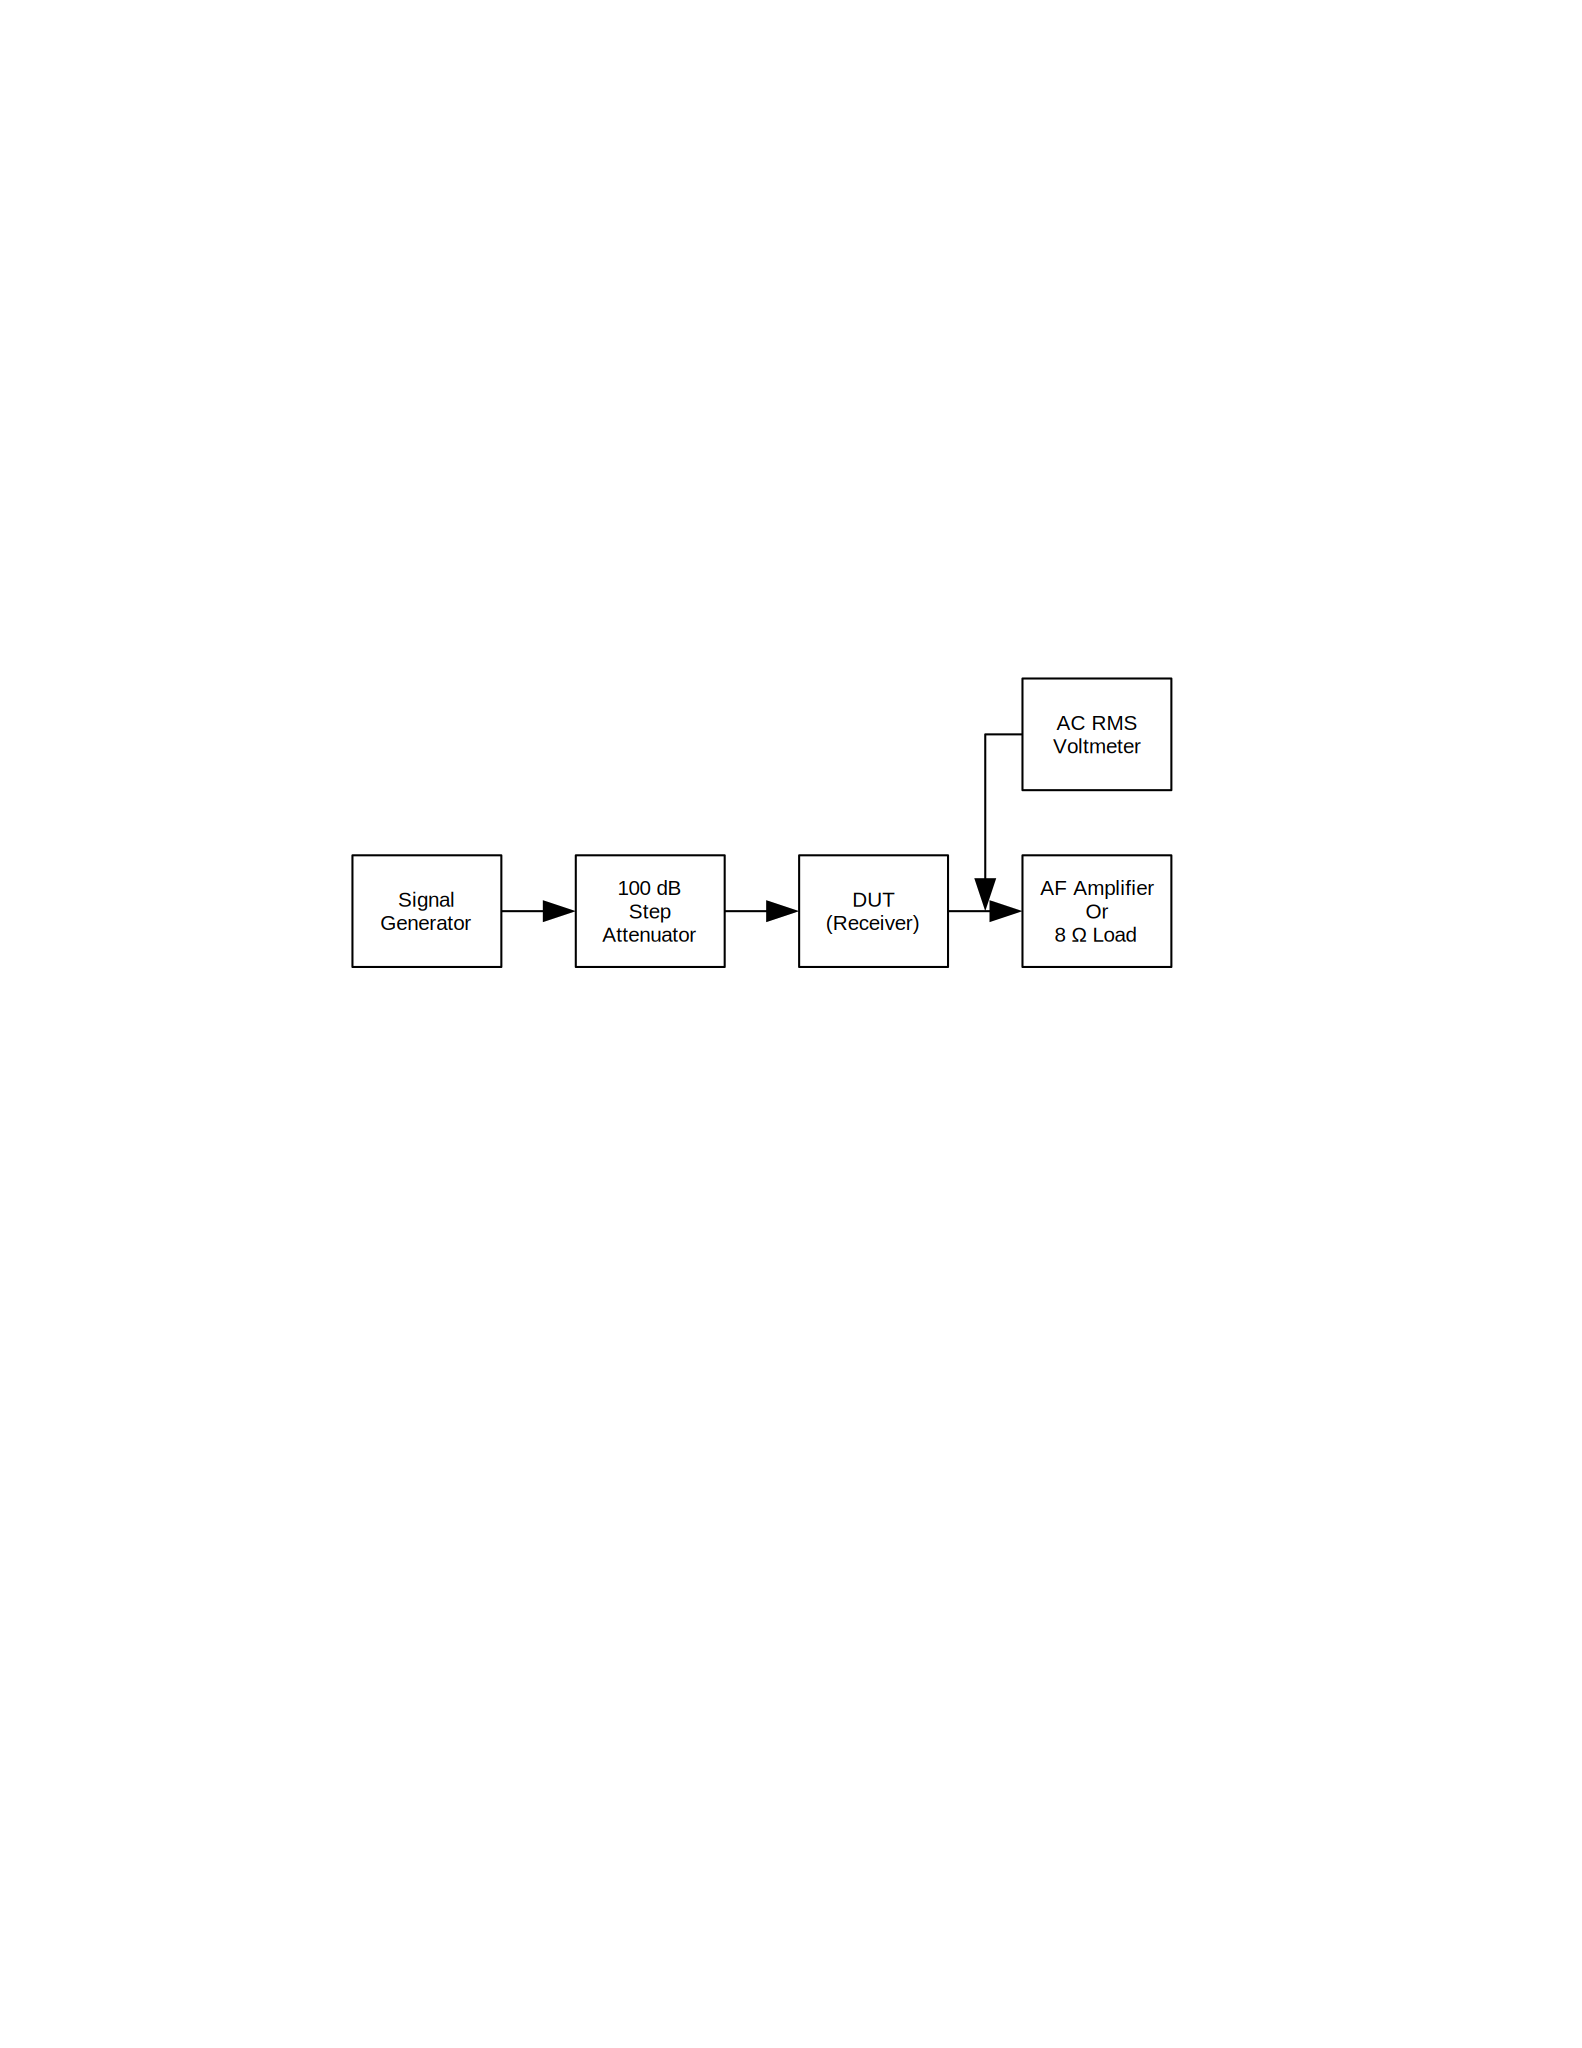
\includegraphics[scale=1]{Illustrations/MDSSetup}
\caption{IF Rejection Setup}
\end{figure}
\subsubsection*{Required Cabling}
\begin{itemize}
	\item 2 --- 50 $\Omega$ jumper cables \vspace{30pt}
		Usually BNC Male-to-BNC Male
	\item 1 --- audio jumper cable \vspace{30pt}
		Varies depending on the connectors on your receiver and AF amplifier or load
	\item 1 --- set of voltage probe test leads \vspace{30pt}
		Your choice of connector for measuring AC RMS voltage output
\end{itemize}
\subsubsection*{Connections}
\emph{Make sure all equipment is powered off before making any connections.}
\begin{itemize}
	\item Connect the signal generator output to one port of the step attenuator using a 50 $\Omega$ jumper cable.
	\item Connect the other port of the step attenuator to the DUT (receiver) using a 50 $\Omega$ jumper cable.
	\item Connect the audio output of the DUT (receiver) to the AF amplifier or 8 $\Omega$ load using an audio jumper cable.
	\item Connect the AC RMS voltmeter probes to the properly loaded audio output of the DUT (receiver).
\end{itemize}
\subsubsection*{Presets}
\begin{itemize}
	\item Turn ON the signal generator but make sure that the output is OFF. Set the output level to -30 dBm (if you are able to). Set the output frequency to the desired test frequency.
	\item Set the step attenuator for -40 dB. This will give an initial test signal level of -70 dBm. If you are not able to set your signal generator to -50 dBm, set the step attenuator to give you -70 dBm of test signal output.
	\item Turn ON the AF amplifier.
	\item Turn ON the DUT (receiver) and set for the desired measurement band and frequency. Set the AF gain (volume) control fully-counterclockwise (no AF output), then set to an appropriate level for normal listening. If your receiver has AGC, disable it.
	\item Turn ON the AC RMS voltmeter. Set the meter scale as necessary.
\end{itemize}

\subsection*{Test Procedure}
\begin{enumerate}
	\item Turn ON the signal generator output and reduce the attenuation. You should hear a CW tone from the AF amplifier. Adjust the frequency so the tone is sentered in the receiver's passband. \vspace{30pt} \vspace{30pt} \vspace{30pt}
	IF center frequency $\rule{3cm}{0.1mm}$ MHz.

	\item Turn OFF the signal generator output.

	\item Note the reading of the AC RMS voltmeter in dB. If the meter reading is fluctuating quite a bit, you may need to increase the AF gain control of the DUT (receiver) in order to get a more stable reading. \vspace{30pt} \vspace{30pt} \vspace{30pt}
	AF noise power $\rule{3cm}{0.1mm}$ 

	\item 4. The IF rejection power level will be the AF power level 3 dB higher than the measurement made in step 4. Calculate it below.\vspace{30pt} \vspace{30pt} \vspace{30pt}

AF Noise + IF rejection power level $\rule{3cm}{0.1mm}$ 

	\item Turn ON the signal generator output. The reading from the AC RMS voltmeter should be significantly higher than the calculated level in step 4 . Use the controls on the step attenuator to step down the test signal level until you have a reading on the AC RMS voltmeter that is closest to the figure derived in step 4. Note the amount of attenuation set on the step attenuator, then subtract that from the output level of the signal generator. This is your IF rejection power level in dBm.\vspace{30pt} \vspace{30pt} \vspace{30pt}
	 IF rejection power: $\rule{3cm}{0.1mm}$ dBm.
	 
	\item 6. The total IF rejection is now calculated by subtracting the IF rejection power level from the MDS of the receiver. \vspace{30pt} \vspace{30pt} \vspace{30pt}
	 IF rejection: $\rule{3cm}{0.1mm}$ dB.


	\emph{For example, if your signal generator is set to 0 dBm and the step attenuator is set to 43 dB, then your IF rejection power level is -43dBm. With an receiver MDS of -131dBm the IF rejection will then be: -43dbm -(-131dBm)=88dB.}
\end{enumerate}

\subsection*{Hints and Tips}
\begin{itemize}
	\item Many QRP receivers and transceivers have a relatively low-level audio output, designed for either headphones-only or for a small speaker. In order to make the most accurate measurement, you may need to turn the AF gain control to maximum.
	\item If the noise vary to much for your readings to be stable, a low pass integrating filter will smooth out the noise and give a stable reading. A suitable filter is a resistor of 10k in series with the signal lead and a 1µF capacitor, if the noise vary to much increase the capacitor to 10µF.  
	\item The IF rejection is the product of the mixer balance and the filter attenuation. Improving the mixer balance will improve the IF rejection.
\end{itemize}





\section{Image Rejection}
\section{Opposite Sideband Rejection}
\section{Two-Tone Third Order Dynamic Range}
\section{Blocking Gain Compression}
\section{Noise Figure}
%This is quite easy to do, will make the text later
Noise figure measurment have the advantage of it being independent on the bandwith of the receiver. The MDS can then be calculated from the bandwith of the receiver.
\subsection*{Equipment List}
\begin{itemize}
	\item Noise source with known output noise (ENR).
	\item AC RMS Voltmeter (preferably with dB scale)
	\item AF Monitor Amplifier or 8 $\Omega$ Resistive Load
\end{itemize}
\subsection*{Test Setup}
\begin{figure}
\centering
\includegraphics[scale=1]{Illustrations/nooisefigure}
\caption{Noise figure Setup}
\end{figure}
\subsubsection*{Required Cabling}
\begin{itemize}
		\item 2 --- 50 $\Omega$ jumper cables \vspace{30pt}
		Usually BNC Male-to-BNC Male
	\item 1 --- audio jumper cable \vspace{30pt}
		Varies depending on the connectors on your receiver and AF amplifier or load
	\item 1 --- set of voltage probe test leads \vspace{30pt}
		Your choice of connector for measuring AC RMS voltage output
\end{itemize}
\subsubsection*{Connections}
\emph{Make sure all equipment is powered off before making any connections.}
\begin{itemize}
\item Connect the noise source to the receiver input, avoid using excessive coax cables and adapters if possible.
\item Connect the other port of the step attenuator to the DUT (receiver) using a 50 $\Omega$ jumper cable.
	\item Connect the audio output of the DUT (receiver) to the AF amplifier or 8 $\Omega$ load using an audio jumper cable.
	\item Connect the AC RMS voltmeter probes to the properly loaded audio output of the DUT (receiver).
\end{itemize}
\subsubsection*{Presets}
\begin{itemize}
	\item Turn OFF the noise source.
	\item Turn ON the AF amplifier.
	\item Turn ON the DUT (receiver) and set for the desired measurement band and frequency. Set the AF gain (volume) control fully-counterclockwise (no AF output), then set to an appropriate level for normal listening. If your receiver has AGC, disable it.
	\item Turn ON the AC RMS voltmeter. Set the meter scale as necessary
\end{itemize}
\subsection*{Test Procedure}
\begin{enumerate}
\item  Record the amplitude in dB of the noise from the receiver with the noise source off.  \vspace{30pt} \vspace{30pt} \vspace{30pt}
	AF noise power $\rule{3cm}{0.1mm}$ dB/mV.
	\item Turn on the noise source and let the output stabilize.
	\item Record the amplitude in dB of the noise from the receiver with the noise source on. \vspace{30pt} \vspace{30pt} \vspace{30pt}
	AF noise power $\rule{3cm}{0.1mm}$ dB/mV.
	\item The ratio of the noise with the noise source on to off is the Y factor. If the measurements of the noise are in dB, the Y factor is: $ Y(dB) = dB(on) - dB(off)$ If the measurement of the noise are in mV then the Y factor is: $ Y = \frac{on(mV)}{off(mV)} $
\item For the noise figure calculation in dB the noise figure is: $ ENR(dB) - Y(dB) $
	\item For the noise figure calculations, the calculation is different if the measurements are done in dB or in Volt. This is due to how multiplications are done with logarithms.
	\item for mV:  $ f = \dfrac{ENR}{Y-1} $ usualy we give noise figure in dB, so in this case: $ NF = 20 \cdot \log(f) $
	\item 
	\item from the noise figure, the MDS can be calculated: $ MDS(dBm) = -174dBm + 10 \log(BW) + NF $ 
\end{enumerate}

\subsection*{Hints and Tips}
\begin{itemize}
\item
\end{itemize}


\section{Audio Frequency Response}
\section{Audio Power Output}

\chapter{Transmitter Measurements}
blah
\section{Transmitter Power Output}
\section{Transmitter Spectral Purity}
\section{Transmitter Carrier and Unwanted Sideband Suppression}
\section{Transmitter Two-Tone Intermodulation Distortion (IMD)}
\section{Transmitter CW Keying Waveform}
\chapter{Components and Circuits}
bluh
\section{Crystal Parameters}
%lots of choises here

\subsection*{Overview method 1}
This method of measuring crystal parameters utilize the fact that a crystal have both a series resonance and a parallel resonance. The frequency of these are measured and the crystal parameters are then calculated. This (should) gives an improved accuracy compared to simpler methods. 
\subsection*{Equipment List}
\begin{itemize}
	\item RF Signal Generator, DDS or synthesized with 1Hz tuning step.
	\item Crystal measurement jig as described under DIY equipment.
	\item RF RMS Voltmeter or power meter(preferably with dB scale, HP3400 or HP432 recomended.) 
	\item 100$\Omega$ non inductive trim potentiometer
\end{itemize}

\subsection*{Test Setup}
\begin{figure}
\centering
\includegraphics[scale=1]{Illustrations/crystals}
\caption{Crystal parameter measurment}
\end{figure}}
\subsubsection*{Required Cabling}
\begin{itemize}
	\item 2 --- 50 $\Omega$ jumper cables \vspace{30pt}
		Usually N Male-to-N Male
	\item 1 --- Adapter \vspace{30pt}
		Varies depending on the connectors on your generator and meter.
	
\end{itemize}
\subsubsection*{Connections}
\emph{Make sure all equipment is powered off before making any connections.}
\begin{itemize}
\item connect the signal generator to the series jig.
\item connect the RF RMS voltmeter or power meter to the series jig.
\end{itemize}
\subsubsection*{Presets}
\begin{itemize}
\item Set signal generator to 0dBm ( 1mW). Most crystals will get damaged at higher power levels.
\item connect a wire, as short as possible over the crystal connections, and note the meter reading. This is your 0dB level. For the short, one can also use the shunt jig without any wire connected. \vspace{30pt} \vspace{30pt} \vspace{30pt}
	 Calibration level: $\rule{3cm}{0.1mm}$ 
\end{itemize}
\subsection*{Test Procedure}
\begin{enumerate}
\item Measure the parasitic package capacitance of the crystal. This should be done on a frequency far away from the crystal frequency, most meters measure this in the 100KHz range. 
\item  measure series resonance freq in series jig by inserting the crystal and finding the frequency where the amplitude read on the meter is max. This frequency is your series frequency F_{S}.  \vspace{30pt} \vspace{30pt} \vspace{30pt}
	F_{S : $\rule{3cm}{0.1mm}$ Hz.
	
\item remove the crystal and insert an 100$\Omega$ trim potentiometer. Adjust this to the same amplitude level as measured for the series connection. Remove the potentiometer and use an ohm meter to measure the resistance. This is your R_{S} resistance.\vspace{30pt} \vspace{30pt} \vspace{30pt}
	R_{S} : $\rule{3cm}{0.1mm}$ $\Omega$. % this resistance can be calculated as well, I just need to derive that exact math, its something like (Z0/2 * dB/1-dbcal)
\item measure parallel resonance freq. in shunt jig by inserting the crystal and finding the frequency where the amplitude read on the meter is max. This frequency is your parallel frequency F_{P}. \vspace{30pt} \vspace{30pt} \vspace{30pt}
	F_{P} : $\rule{3cm}{0.1mm}$ Hz.
\item do some math on the data, flush and repeat.. 
\item The crystal motional series capacitor $C_{m}$ is found by calculation: \vspace{30pt} $ C_{m} = C_{p}\cdot\frac{F_{p}^{2}-F_{s}^{2}}{F_{s}^{2}} $
\item then the inductance can be found: $ L_{m} = \dfrac{1}{c_{p}\cdot 4 \cdot \pi^{2} \cdot F_{p}^{2}-F_{s}^{2} } $
\item The Q factor of the crystal can then be found: $ Q = \frac{L_{m}\cdot 2 \cdot \pi \cdot F_{s}}{R_{s}}   $

\item With these calculations done, the crystal parameters are characterized. The accuracy of the frequency measurement is what defines the accuracy of this method. 

\end{enumerate}

\subsection*{Hints and Tips}
\begin{itemize}
\item An automated test for this can be done with computer controlled equipment, and the crystal parameters can then be calculated automatic. This is the method most network analyzers use for characterizing crystals.
\end{itemize}





\section{Third-Order Intercept}
\section{Noise Figure}
% this depeends opon what equipment are avaible and what component to be measured, could be its own chapter.
\subsection*{Overview method 1}
%things
\subsection*{Equipment List}
\begin{itemize}
	\item items
\end{itemize}
\subsection*{Test Setup}
\begin{figure}
\centering
\includegraphics[scale=1]{Illustrations/noisefigure}
\caption{Noise figure Setup}
\end{figure}
\subsubsection*{Required Cabling}
\begin{itemize}
	\item 2 --- 50 $\Omega$ jumper cables \vspace{30pt}
		Usually BNC Male-to-BNC Male
\end{itemize}
\subsubsection*{Connections}
\emph{Make sure all equipment is powered off before making any connections.}
\begin{itemize}

\end{itemize}
\subsubsection*{Presets}
\begin{itemize}

\end{itemize}
\subsection*{Test Procedure}
\begin{enumerate}
\item  
\end{enumerate}

\subsection*{Hints and Tips}
\begin{itemize}
\item
\end{itemize}


\section{Resonator Q}
% here there are several metthods, we should probably describe them all, as not all are suitable for all components
\chapter{DIY Test Equipment}
\section{crystal measurement jig}
\begin{itemize}
\item Cut 2 traces in a PCB (or order it from OSHpark: https://oshpark.com/shared_projects/Ert6eRmg )

\item  Fit 2 pices of an IC socket to it so you keep the 50 ohm environement but it allows for measurment of crystals.
\item Use good sockets, goldplated prefered.  
\end{itemize}
\section{Noise Figure stuff}
blah
\end{document}